\hmsubsection{Image Processing Pipeline}{OAH}{}

This section describes the image processing pipeline responsible for detecting
and classifying red and blue balls in each frame captured by the OAK Series~2
camera. The pipeline is implemented in the \texttt{SimpleBallDetector} class
and executed once per frame in the following order: image acquisition, image preprocessing, adaptive
lighting compensation, HSV colour segmentation, Hough
Circle Transform, ensemble merging, and object tracking. Each stage is
described in the subsections below.

\hmsubsubsection{Image Acquisition}{OAH}{}

Image acquisition is handled by the OAKCamera class, which wraps the
Luxonis OAK Series~2 camera through the DepthAI v3~API\@. The camera is equipped
with a Sony IMX378 RGB sensor and an onboard Movidius MyriadX VPU, connected to
the Raspberry Pi~5 via USB~3.

The OAKCamera class exposes a read()/release() interface compatible with OpenCV's
VideoCapture, which decouples the rest of the image processing pipeline from the
specific hardware used. Frames are delivered as NumPy arrays in BGR format at a
configured resolution of $640 \times 400$ pixels.

Upon initialisation, the camera discards the first 30 frames before making itself
available for use. This warmup period is required because the camera's automatic
exposure (AE) and automatic white balance (AWB) algorithms have not yet converged
at startup. Without this step, the initial frames exhibit a mean brightness of
approximately 32/255, rendering them unsuitable for colour-based detection. This
issue was particularly pronounced when operating over USB~2.0 connections.

The focal length in pixels, required for distance estimation, is retrieved from the
camera's factory-calibrated intrinsics stored in EEPROM via the DepthAI API\@. If
calibration data is unavailable, the focal length is derived theoretically from the
horizontal field of view ($\mathrm{HFOV} = 81^{\circ}$) using the pinhole camera
model:
\begin{equation}
    f = \frac{w/2}{\tan\!\left(\dfrac{\mathrm{HFOV}}{2}\right)}
\end{equation}
where $w$ is the image width in pixels.

\hmsubsubsection{Adaptive Lighting Compensation}{OAH}{}

Variations in ambient lighting represent a significant challenge for colour-based object
detection. To address this, the system incorporates an adaptive lighting compensation module
consisting of two stages: lighting analysis and image enhancement. Both stages operate on the
downscaled frame produced in the preprocessing step.

In the first stage, the mean pixel brightness of the downscaled frame is computed from its
grayscale representation. Based on this value, the lighting condition is classified into one of
three levels: low (mean brightness below 100), medium (between 100 and 140), and high (above
140). These thresholds correspond approximately to an estimated illuminance range of 300--700
lux, derived from the linear mapping:
\begin{equation}
    E_{\text{lux}} = \text{clip}\!\left(300 + (\bar{I} - 80) \cdot 4.0,\ 300,\ 700\right)
\end{equation}
where $\bar{I}$ is the mean pixel intensity on a scale of 0--255.

In the second stage, Contrast Limited Adaptive Histogram Equalisation (CLAHE) is applied
unconditionally to every frame, regardless of the detected lighting level. The image is first
converted from BGR to the LAB colour space, after which CLAHE is applied exclusively to the
L-channel with a clip limit of 2.5 and a tile grid size of $8 \times 8$ pixels. The frame is
then converted back to BGR before further processing. This approach enhances local contrast
without distorting the colour information contained in the A and B channels, which are used in
subsequent detection stages.

Applying CLAHE to all frames, rather than only under low-light conditions, was found to be
necessary because uneven illumination — such as vignetting and localised shadows from the
robot arm — produces dark regions even under nominally adequate lighting. By normalising
contrast locally on every frame, the fixed HSV colour thresholds remain effective across the
full operating range without any dynamic threshold adjustment.

\hmsubsubsection{Image Preprocessing}{OAH}{}

Prior to colour segmentation, each incoming frame undergoes a series of
preprocessing steps to reduce computational load and improve detection robustness.

The first step is spatial downscaling. Each frame is resized to 75\% of its
original dimensions using bilinear interpolation, producing a processing resolution
of $480 \times 300$ pixels from the input resolution of $640 \times 400$ pixels.
This scale factor was chosen to balance processing speed with sufficient spatial
resolution for shape-based validation. At this scale, the ball radius is
approximately 11 pixels, which provides enough structural detail for the subsequent
morphological and contour operations. A scale factor of 0.5 was evaluated but
rejected, as the resulting ball radius of approximately 7 pixels caused the
$13 \times 13$ closing kernel to span 87\% of the ball diameter, destroying the
shape features required by the geometric gate filters. The radius thresholds used
for contour validation are scaled proportionally to match the reduced coordinate
space.

Following downscaling, the frame is converted from BGR to HSV colour space for
colour segmentation, and separately to grayscale for geometric operations. A
Gaussian blur with a $5 \times 5$ kernel is applied to the grayscale
representation to suppress high-frequency noise, as illustrated in
Figure~\ref{fig:gaussian_blur}. The HSV representation is not blurred, as the
colour segmentation masks are subsequently filtered through morphological
operations.

\begin{figure}[h]
\centering
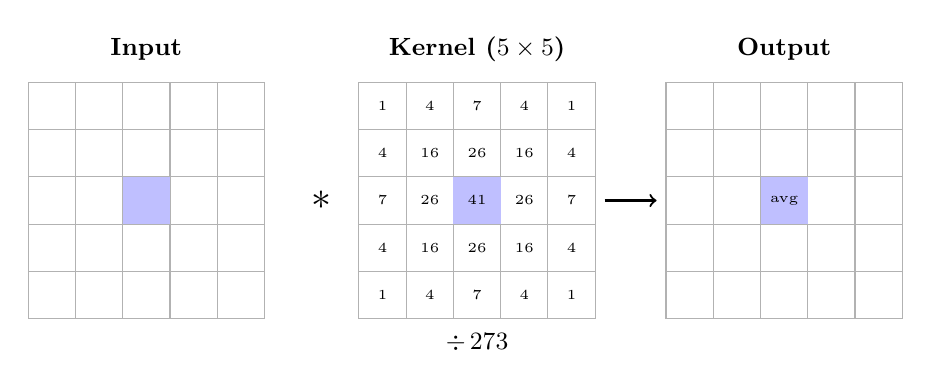
\begin{tikzpicture}[scale=0.6]

% --- Input grid (5x5) ---
\foreach \i in {0,...,4} {
    \foreach \j in {0,...,4} {
        \draw[gray!60] (\i,\j) rectangle (\i+1,\j+1);
    }
}
\fill[blue!25] (2,2) rectangle (3,3);
\node[font=\small\bfseries] at (2.5, 5.7) {Input};

% --- Convolution symbol ---
\node[font=\Large] at (6.2, 2.5) {$*$};

% --- Kernel grid (5x5) with values ---
\foreach \i in {0,...,4} {
    \foreach \j in {0,...,4} {
        \draw[gray!60] (7+\i,\j) rectangle (7+\i+1,\j+1);
    }
}
\fill[blue!25] (9,2) rectangle (10,3);

\foreach \i/\j/\val in {
    0/4/1, 1/4/4,  2/4/7,  3/4/4,  4/4/1,
    0/3/4, 1/3/16, 2/3/26, 3/3/16, 4/3/4,
    0/2/7, 1/2/26, 2/2/41, 3/2/26, 4/2/7,
    0/1/4, 1/1/16, 2/1/26, 3/1/16, 4/1/4,
    0/0/1, 1/0/4,  2/0/7,  3/0/4,  4/0/1
}{
    \node[font=\tiny] at (7+\i+0.5, \j+0.5) {\val};
}
\node[font=\small\bfseries] at (9.5, 5.7) {Kernel ($5\times5$)};
\node[font=\small] at (9.5, -0.5) {$\div\,273$};

% --- Arrow ---
\draw[->, thick] (12.2, 2.5) -- (13.3, 2.5);

% --- Output grid (5x5) ---
\foreach \i in {0,...,4} {
    \foreach \j in {0,...,4} {
        \draw[gray!60] (13.5+\i,\j) rectangle (13.5+\i+1,\j+1);
    }
}
\fill[blue!25] (15.5,2) rectangle (16.5,3);
\node[font=\tiny] at (16.0, 2.5) {avg};
\node[font=\small\bfseries] at (16.0, 5.7) {Output};

\end{tikzpicture}
\caption[Gaussian blur with a $5 \times 5$ kernel.]{Gaussian blur with a $5\times5$
kernel. Each output pixel (highlighted) is computed as the weighted sum of its
neighbourhood, divided by 273. Pixels closer to the centre receive higher weights.
High-frequency noise is suppressed because isolated bright or dark pixels are
averaged with their neighbours.}
\label{fig:gaussian_blur}
\end{figure}